\documentclass[../main]{subfiles}
\begin{document}

\section{
  Brainfuck parsing and code generation
}

Now that we introduced the various techniques to generate programs from
pointer trees generated by \constexpr functions, we will use them in the
context of compile-time parsing and code generation for the Brainfuck language.
Therefore use data structures and code generation techniques introduced in
subsection \ref{lbl:ptr-tree-codegen}.

\subsection{
  Constexpr Brainfuck parser and AST
}

\subsubsection{
  Parser
}

\subsubsection{
  AST
}

\subsubsection{
  Difficulties
}

\begin{itemize}
\item Embedding text from the original string
\end{itemize}


\subsubsection{
  Implementation complexity
}

\subsubsection{
  Small synthetic variable-size benchmarks
}

We first begin by running two variable-sized benchmarks, consisting in
measuring compiler execution time as the AST widens, and as the AST deepens.

The first variable-sized benchmark consists in generating a valid BF AST by
concatenating strings to generate a succession of BF while loops in a
\constexpr string. This benchmark was instantiated with sizes going from 1 to
10 with a step of 1, with 10 timing iterations for each size.

The second benchmark generates a string with
nested loops, making the AST deeper as the benchmark size increases instead
of making it wider as in the previous case.

Both benchmarks generate programs of the same size so comparisons can be made
properly.

\begin{figure}
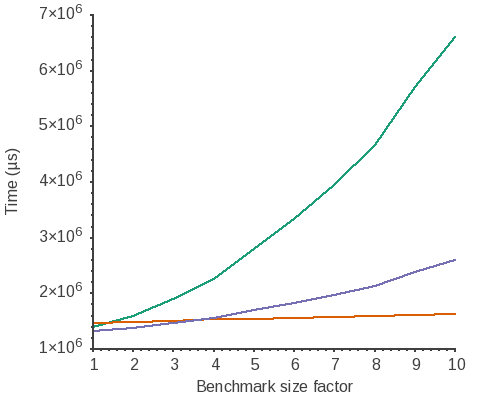
\includegraphics[scale=0.5]{images/bf-consecutive_loops.png}
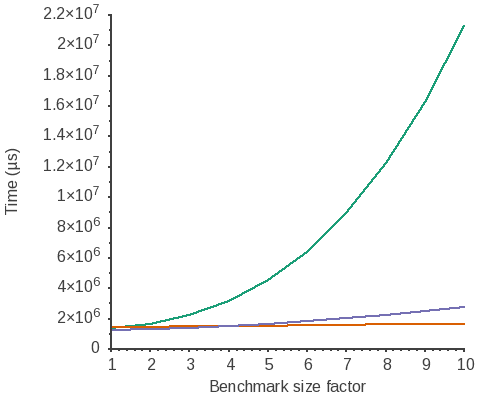
\includegraphics[scale=0.5]{images/bf-imbricated_loops.png}
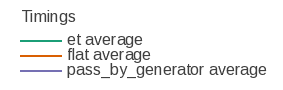
\includegraphics[scale=0.5]{images/bf-graph-legend.png}
\caption{
  Compiler execution time measurements for consecutive loops (left)
  and nested loops (right)
}\label{fig:bf-bench}
\end{figure}

Figure \ref{fig:bf-bench}
both highlight considerably higher compiler execution times for the expression
template based backend, high enough to suggest that the use of expression
templates induces an overhead higher than parsing and generating Brainfuck
programs using the pass-by-generator backend. However the pass-by-generator
backend still has a compile time overhead much higher than the flat backend,
which shows near constant compiler execution times on these small scale
benchmarks.

Finally, AST deepening has a much higher impact on compile times than AST
widening with the expression template backends, whereas the other backends seem
to scale similarly as the AST grows wider or deeper.

\subsubsection{
  Large Brainfuck programs
}

The following benchmarks consist in measuring compiler execution times for
compiling Brainfuck code examples. These example programs are also used to
validate the metacompiler's backend implementations by compiling them and
verifying their output.

\begin{itemize}
\item A Hello World program (106 tokens).
\item The same Hello World program, ran twice (212 tokens).
\item A Mandelbrot set fractal viewer (11672 tokens).
\end{itemize}

\begin{figure}
\begin{tabular}{|c|c|c|c|}
\hline
Backend             & Hello World & Hello World x2  & Mandelbrot \\
\hline
Flat                & 1.81        & 2.25            & 49.68 \\
Pass-by-generator   & 9.77        & 34.37           & Failure (timeout) \\
Expression template & 50.60       & 192.73          & Failure (timeout) \\
\hline
\end{tabular}
\caption{BF compile time measurements in seconds
}\label{fig:BF-compile-times}
\end{figure}

The measurements in figure \ref{fig:BF-compile-times} help us better understand
how various metacompiling techniques behave at scale. The "Flat" backend shows
very good performance on all examples, including the Mandelbrot example that is
about 100 times larger than the Hello World example. However the other cases
highlight severe scaling issues and tend to confirm our previous hypothesis
being that using generator functions to pass values makes the code generation
quadratic. Finally, the "Expression template" backend performance highlights
heavy performance impact when expression templates are being used, which is
likely due to the complexity of the mechanisms expression templates involve like
SFINAE and overload resolution.

\subsubsection{
  Conclusions
}

\end{document}
